\section{Discussion} \label{sec: discussion}
\textbf{The flexibility of agentic frameworks.} A key advantage of agentic frameworks over fixed approaches is their adaptability to specific tasks. Table \ref{tab:extraction_steps_comparison} illustrates how phenotype and disease extraction agents use different tools and implementations while following the same core workflow of extract, verify, match, and refine. Each agent can be customized—for example, including abbreviation detection or lab event databases for phenotype extraction while omitting lab events for rare disease extraction, where they provide no value. Expanding the available tool set, such as incorporating medical knowledge graphs, could further enhance phenotype reasoning performance.

\textbf{Improving medical reasoning.} A key limiting factor in LLMs becoming more useful for phenotype and rare disease mention mining is their inability to reason medically about various observed conditions, as such details are often implicit. While there is extensive work on differential diagnosis \cite{chen2024rarebenchllmsserverare,chen2025rareagentsadvancingraredisease, germain2025applyingAI_RD}, LLMs remain insufficient for basic reasoning tasks like implying phenotypes related to lab events and other key indicators within the text as shown by the tiny improvements to extraction performance in Table \ref{tab:rdma_ablation} when adding a phenotype implication step. Existing medical reasoning works are still new and often fail to encompass the reasoning steps taken by clinicians, especially rare disease specialists, due to the scarcity and sparsity of existing knowledge surrounding rare conditions. Expecting LLMs to understand and perform differential diagnosis without being able to extract all phenotypes or rare disease mentions would be premature.

\textbf{Constructing more publicly available rare disease datasets.} Current datasets for mining rare diseases and phenotypes \cite{lobo2017identifying_human_phenotype_terms,garcia2024_HPORAG,dong2023ontology_poor_annotations,martínezdemiguel2021rarediscorpuscorpusannotated} have several drawbacks in benchmarking. Sentence snippets and scientific passages \cite{lobo2017identifying_human_phenotype_terms,martínezdemiguel2021rarediscorpuscorpusannotated} may not reflect the lengthy nature of real-world clinical notes, which often contain thousands of words. Case studies used as benchmarking proxies \cite{garcia2024_HPORAG} lack the noise seen in clinical notes from MIMIC \cite{johnson2016mimic3,johnson2023mimic4}, such as abbreviations and misspellings. Human annotations of rare disease mentions \cite{dong2023ontology_poor_annotations} have been poor due to the required clinical expertise, a problem even in general medical condition annotation tasks like medical coding, where LLMs struggle \cite{soroush2024largelanguagemodelsarePoorMedicalCoders,wang2024drg}. RDMA presents a step forward in being more robust to clinical note lengths, medically-specific abbreviations, and providing a refinement feature to assist clinicians in building more comprehensive rare disease datasets from existing EHRs. However, our new annotations are still small and potentially noisy. With over 6,000 rare diseases in Orphanet \cite{weinreich2008orphanet} and over 15,000 phenotypes in HPO \cite{gargano2024mode_hpo}, datasets are not yet mature enough for training expert models.

\textbf{RDMA in Rare Disease Diagnostics.} We mine rare disease information to better understand their diagnosis. While LLM agents for differential diagnosis are being explored \cite{chen2025rareagentsadvancingraredisease}, their datasets are often limited to a tiny subset of the rare disease space \cite{chen2024rarebenchllmsserverare} or rely on ICD codes as a proxy label for rare diseases \cite{chen2025rareagentsadvancingraredisease}. However, using ICD codes is flawed because they do not capture rare diseases precisely enough \cite{mazzucato2023orphacodes_better}, only cover a subset of rare diseases compared to the Orphanet ontology \cite{kodra2012classification_icd_incomplete}, and approximately 50\% of ICD codes in MIMIC datasets are missing from the text \cite{cheng-etal-2023-mdace}. These challenges lead to an incomplete picture of automated rare disease differential diagnosis. RDMA provides an approach that directly annotates HPO and ORPHA codes for more accurate rare disease profiles.

\textbf{Potential Future of Multimodal Agents in Rare Diseases.} Agents have seen tremendous performance and capability improvements in the past 5 years, especially in incorporating modalities beyond text \cite{wang2024survey_agents}, particularly in the medical domain \cite{sviridov20253mdbenchagent,schmidgall2024agentclinic}. Agentic systems are becoming capable of using lab event diagnostics \cite{wu2024instruction_tuning_multimodal} and images \cite{xia2024cares_medical_vision_language_models} in their judgment. Combined with existing knowledge bases for rare disease diagnosis \cite{nelson2002unified_UMLS}, RDMA could be adapted to mine EHRs beyond text formats, offering a more comprehensive view of patient profiles in rare disease mining.




% move this to the discussion it's redundant.
\rev{\subsection{Key Challenges in Mining}} \label{sec: challenges in mining}

\textbf{A substantial number of phenotypes are implied.} Breaking down the benchmark graciously provided by \cite{garcia2024_HPORAG}, their annotations suggest that over 25\% of the phenotypes are not explicitly mentioned in text as shown in Fig. \ref{fig:DatasetBreakdown}. As a key consequence, LLMs need to be able to directly infer such phenotypes from indicators within the text such as lab events and other combinations of symptoms \cite{wei2015extracting_survey_phenotypes}, not obvious in text. We attempt to extract these implied phenotypes through our implication and verification reasoning steps in step 2 in Fig. \ref{fig:RDMAvRAG} with the usage of a lab events range database. However, despite our improvements with the addition of a lab events database tool, its improvement is not dramatic, suggesting that the vast majority of implied phenotypes are still not being caught as shown in Table \ref{tab:rdma_ablation}. This large presence of implied phenotypes could also explain why all baselines struggle to surpass 65 \% F1 in phenotype extraction.

\begin{figure}[h!]
    \centering
    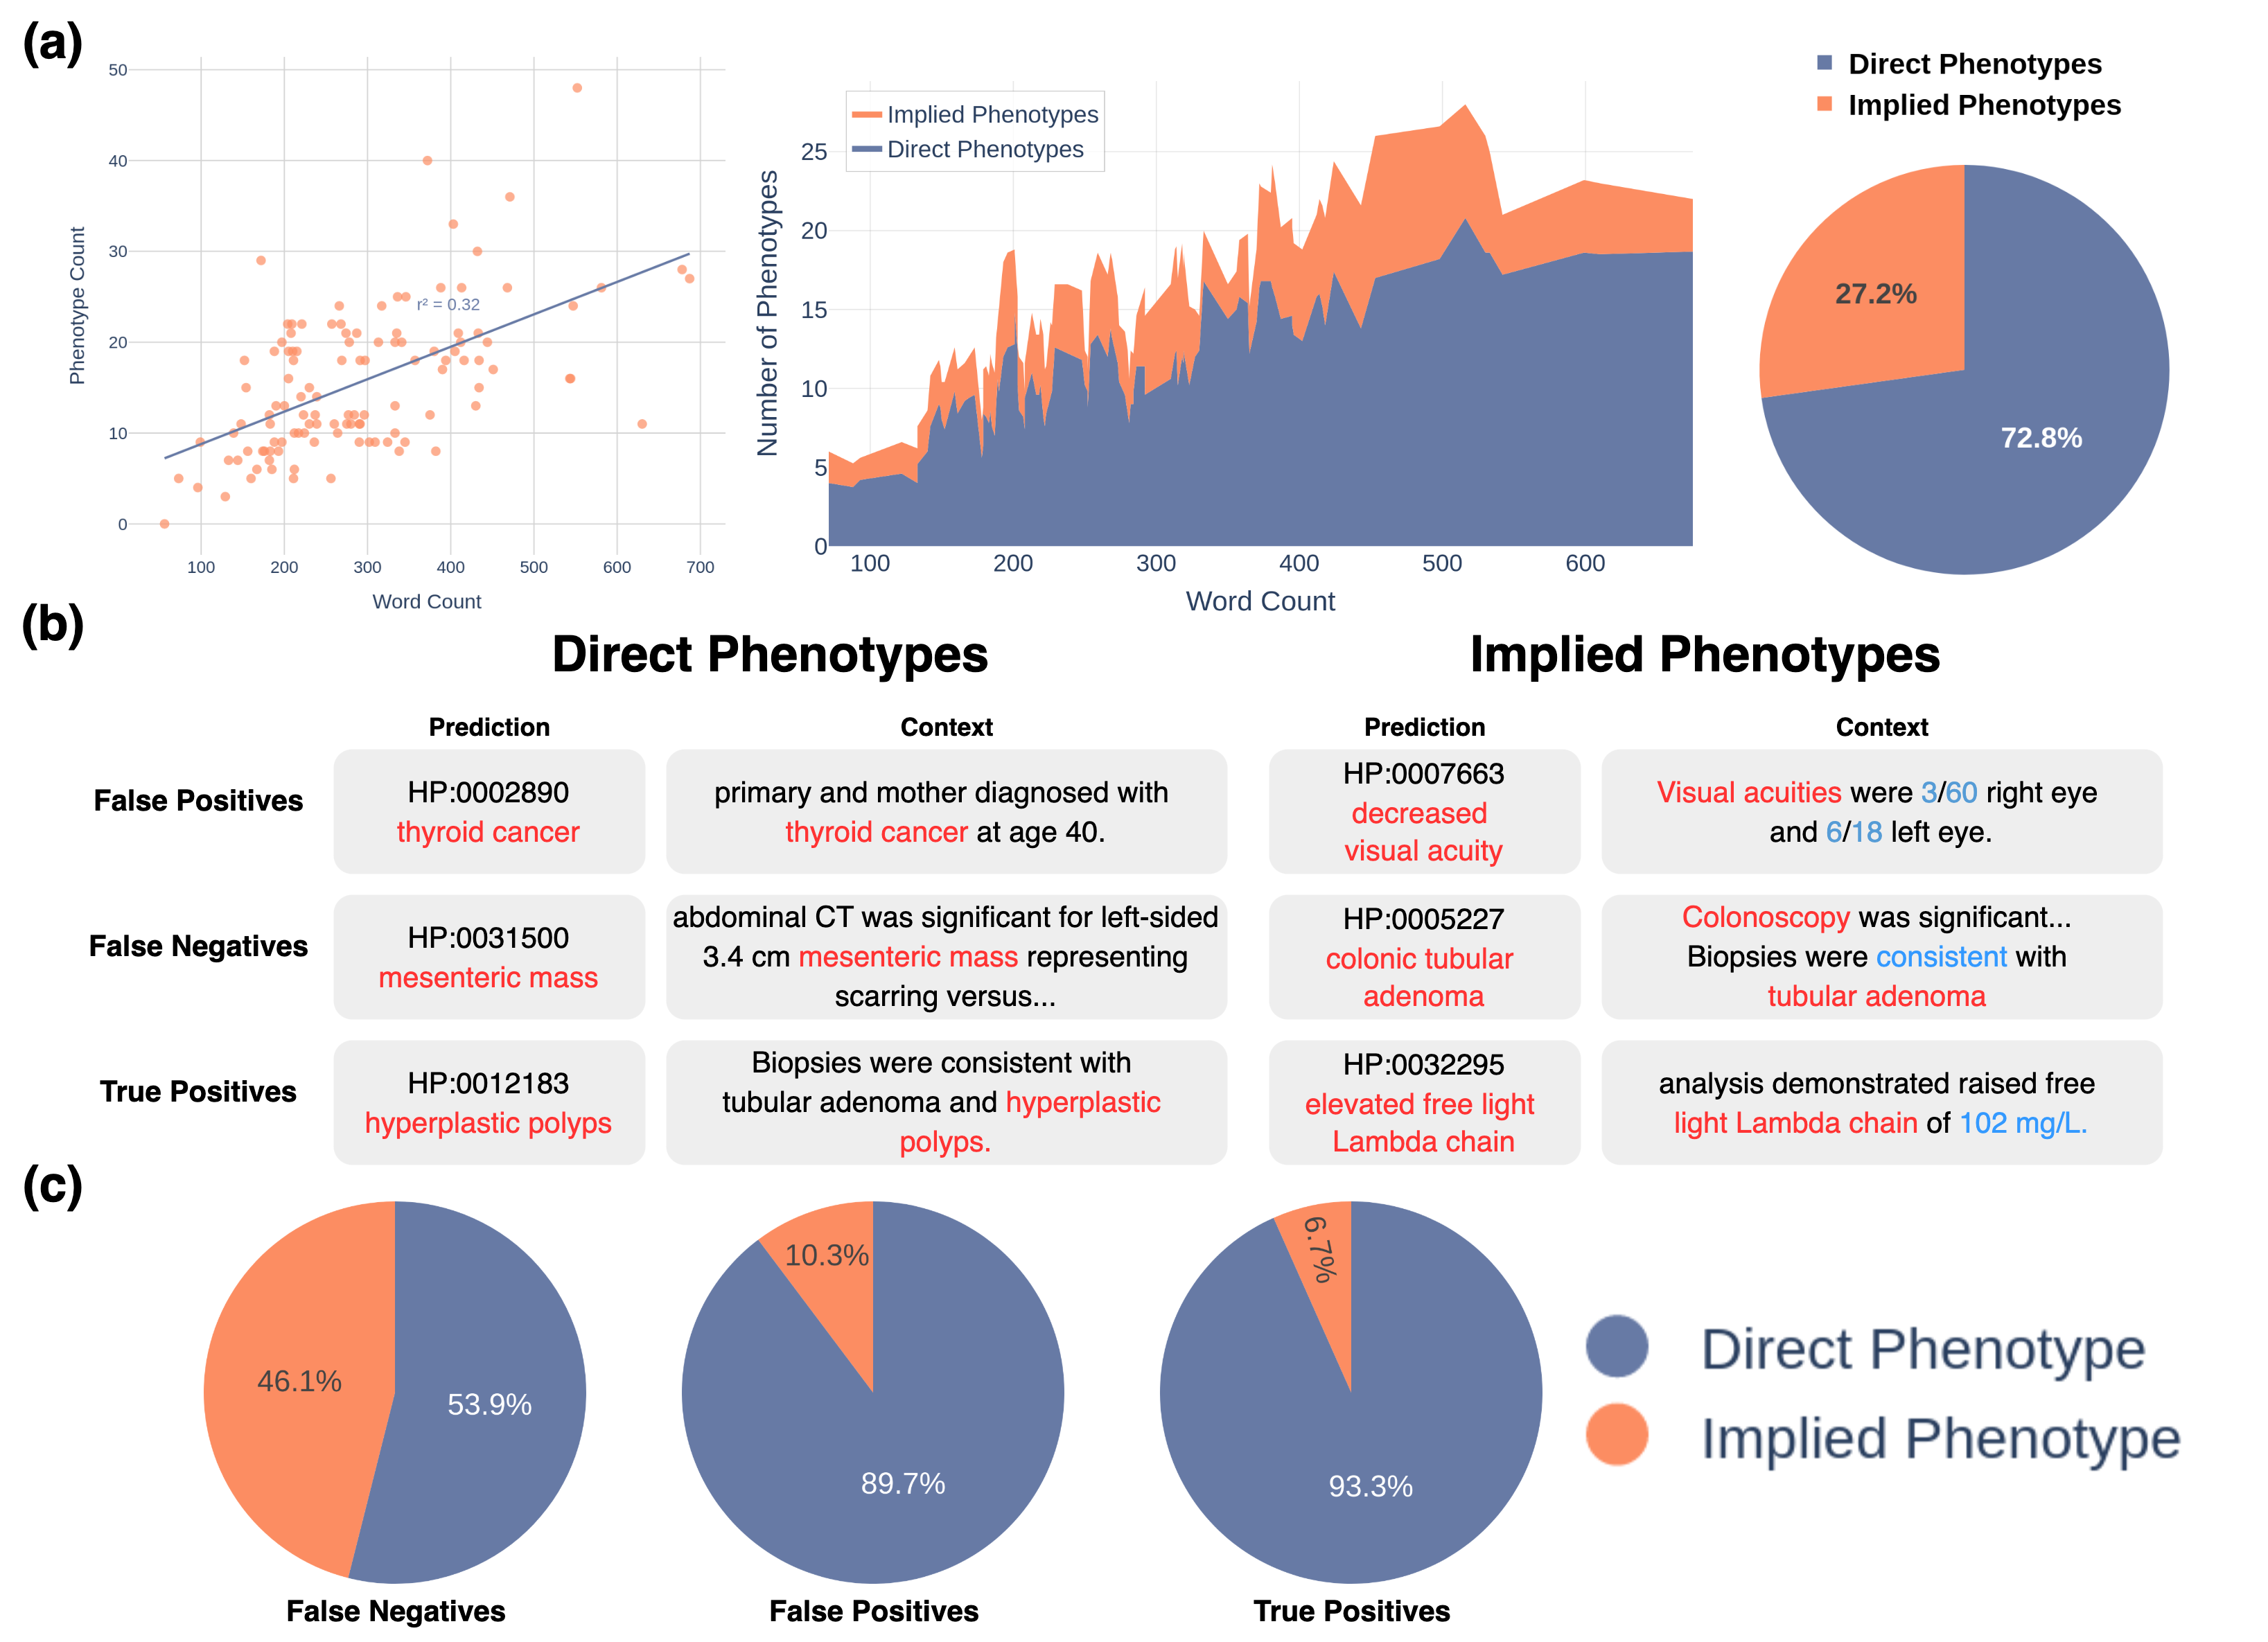
\includegraphics[width=1.0\textwidth]{figs/PhenotypeQualitativeEvaluationsAndStatistics.drawio.png}
    \caption{\textbf{HPO Extraction Evaluation Breakdown.} We evaluate on 116 clinical cases (33,824 words total) from \cite{garcia2024_HPORAG}. \textbf{(a) Dataset Statistics.} Document length weakly correlates with phenotype count. Of 1,813 total phenotypes, 1,320 (72.8\%) appear explicitly in text while 493 (27.2\%) are implied. \textbf{(b) Qualitative Analysis.} Our method captures phenotypes implied by lab tests and related mentions. Key challenges include: (1) False positives that, while not matching labeled HPO codes, are not necessarily incorrect within context—for example, predicting "decreased visual acuity" from impaired vision measurements is clinically valid; (2) False negatives typically arise from missing non-obvious phenotypes like "mesenteric mass" or failing to capture long-range context needed for implied phenotypes like "colonic tubular adenoma," which requires understanding earlier mentions of colonoscopies. Among direct phenotypes, we also observe that there can be cases where the existing label set was not necessarily comprehensive such as "thyroid cancer" not being within the original label set. \textbf{(c) Performance Breakdown.} Though implied phenotypes comprise only 27.2\% of labels, they account for a disproportionate share of false negatives, while most correct predictions are direct phenotypes. }
    \label{fig:DatasetBreakdown}
\end{figure}

\textbf{Clear Challenges in Mining Phenotypes.} To better understand the sources of error, we examine false positive and false negative cases for our phenotypes in Fig. \ref{fig:DatasetBreakdown} (b). Many false positives are not technically incorrect despite lacking the exact code from human annotations. For example, "decreased visual acuity" correctly reflects the eye measurements but does not precisely match the manually annotated HPO code "reduced visual acuity." Conversely, RDMA sometimes identifies direct phenotypes like "thyroid cancer" that human annotators missed, suggesting our method can capture entities overlooked during manual annotation. However, RDMA frequently fails to extract phenotypes that require long-context reasoning or inference from implicit information. This performance gap indicates that agentic systems still face challenges in identifying implied phenotypes. Despite these limitations, our relative performance metrics across all methods align with our brief qualitative observations.


\begin{figure}[h!]
    \centering
    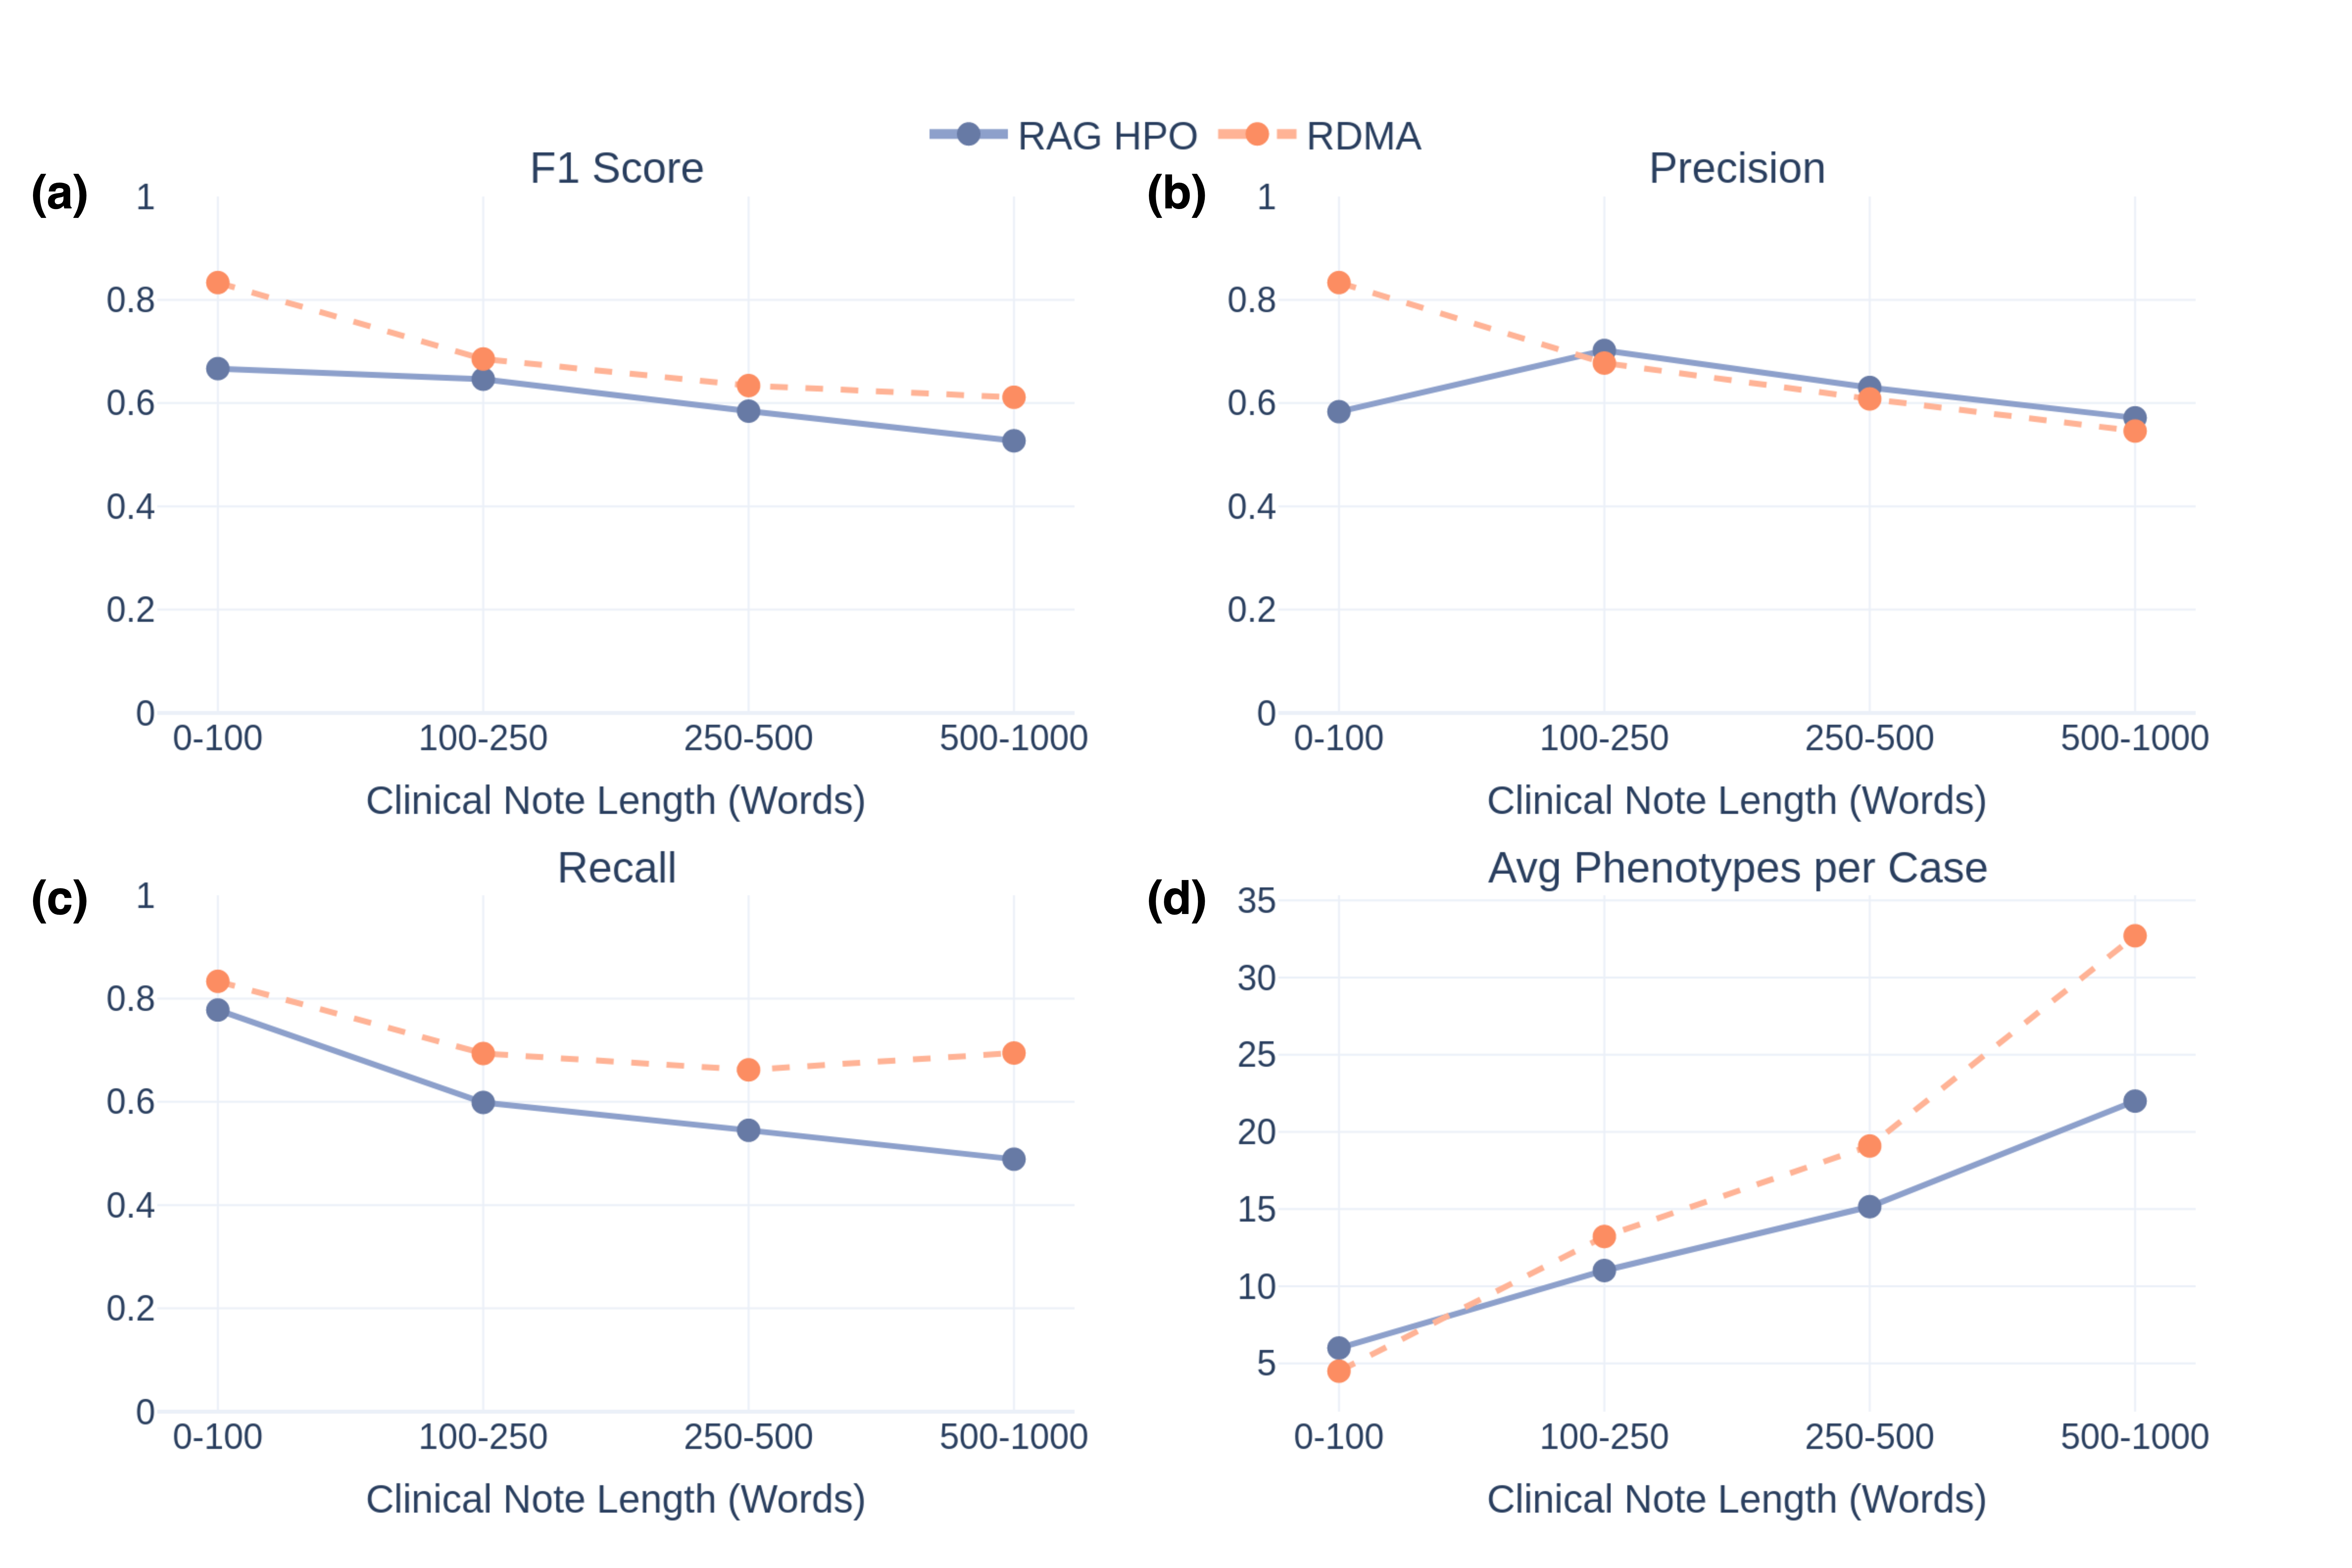
\includegraphics[width=\textwidth]{figs/hpo_metrics_grid_v2.drawio.png}
    \caption{\textbf{RDMA outperforms local RAG-HPO across note lengths.} Real-world clinical notes such as those in MIMIC-IV \cite{johnson2023mimic4_note} are substantially longer than annotated clinical case studies. The median clinical note in MIMIC-IV contains 1,320 words \cite{edin2023automated_medical_coding_survey} compared to 271.5 words in our clinical case study benchmark. Therefore, it is critical that our method maintains reasonable performance across varying note lengths, as the number of phenotypes typically increases with note length (d). While overall precision decreases as note length increases (b), RDMA maintains stable recall performance (c), enabling it to outperform its RAG-based counterpart across all note lengths (a). }
    \label{fig:RDMA_Note_Lengths}
\end{figure}

\textbf{RDMA recall does not degrade as note length increases.} In Fig. \ref{fig:RDMA_Note_Lengths}, we observe that while precision slightly decreases, our overall F1 score appears to flatten out as note lengths increase. Remarkably, our recall slightly increases with longer texts, allowing us to extract more phenotypes as documents grow larger. This suggests that despite some persistent noise (which also affects RAG-HPO approaches), our method demonstrates significantly greater robustness to varying text lengths, ensuring more comprehensive phenotype extraction. We hypothesize this result stems from our approach directly leveraging ontologies within the extraction process—specifically, by retrieving against every sentence and having the LLM agent directly verify whether phenotype-related entities exist within each sentence. In contrast, RAG-HPO approaches typically perform one-shot extraction of the entire document \cite{garcia2024_HPORAG}, explaining why larger models improve performance on these extraction tasks, as increased model size correlates with reduced generation noise \cite{kaplan2020scalinglawsneurallanguage}. Additionally, we instruct our agent to extract anything potentially related to phenotyping, a comprehensive approach not typically employed in RAG-HPO methods.



% \begin{table}[htbp]
%     \centering
%     \begin{tabular}{lccc}
%         \toprule
%         \textbf{Baseline} & \textbf{F1} & \textbf{Precision} & \textbf{Recall} \\
%         \midrule
%         RDMA & \textbf{0.651} & 0.626 & 0.678 \\
%         RDMA (No Lab Test Tool) & 0.636 & 0.628 & 0.644 \\
%         RDMA (No Implication Check) & 0.645 & \textbf{0.640} & 0.650 \\
%         RDMA (No verification) & 0.531 & 0.423 & \textbf{0.710} \\
%         \bottomrule
%     \end{tabular}
%     \caption{\textbf{RDMA Ablation Study.} Comparison of performance differences between additional steps that we improve upon the existing RAG HPO \cite{garcia2024_HPORAG} framework.}
%     \label{tab:rdma_ablation}
% \end{table}
\begin{wraptable}{r}{0.45\textwidth}
    \centering
    \small % Reducing font size slightly helps the table fit in narrow columns
    \begin{tabular}{lccc}
        \toprule
        \textbf{Baseline} & \textbf{F1} & \textbf{P} & \textbf{R} \\
        \midrule
        RDMA & \textbf{0.65} & 0.63 & 0.68 \\
        No Lab Tool & 0.64 & 0.63 & 0.64 \\
        No Impl. Check & 0.65 & \textbf{0.64} & 0.65 \\
        No Verif. & 0.53 & 0.42 & \textbf{0.71} \\
        \bottomrule
    \end{tabular}
    \caption{\textbf{RDMA Ablation Study.} Impact of individual components on phenotype mining performance.}
    \label{tab:rdma_ablation}
\end{wraptable}

\textbf{What matters in RDMA.} We ablate RDMA by systematically removing several key steps in phenotype extraction, including the lab test tool, phenotype implication reasoning, and the verification step. While performance improvements are observed with each of these components, RDMA sees the most significant improvement from its verification step, which dramatically enhances precision. The other steps primarily contribute to improving the model's recall of additional phenotypes. We further discuss some of its implications and future directions in Section \ref{sec: discussion}.

\textbf{Clear Challenges in Mining Rare Diseases.} We observe several challenges when leveraging RDMA, as illustrated in Fig. \ref{fig:annotator_agreement_qualitative}. First, RDMA can be overly strict in rare disease classification, incorrectly rejecting valid rare diseases when they lack exact matches in the Orphanet database. For example, despite having multiple relevant candidates for "portal vein thrombosis" in Orphanet, RDMA may fail to recognize it as a rare disease due to slight terminology differences. Second, RDMA struggles with negation detection, failing to properly interpret phrases like "which was negative" that negate the presence of a condition, despite being explicitly asked in the prompt to consider negations (Fig. \ref{fig:EntityExtractionPrompt}). These challenges stem from limitations in LLMs' ability to perform nuanced reasoning over clinical text.

